\documentclass[hyperref={pdfpagelabels=false, unicode},pdf,slideColor,fyma,9pt]{beamer}
\usepackage[utf8]{inputenc}		%kodovani zdrojoveho textu
\usepackage[czech]{babel} 		%cestina
\usepackage[IL2]{fontenc}		%font vyladeny pro cestinu
\usepackage{lmodern}			%odstraneni varovani pro IL2
\usepackage{graphicx}
\usepackage{color}
\usepackage{multirow}	
\usepackage{subfigure}

\newcommand\myqt[1]{\quotedblbase #1\textquotedblleft}

%cislovani stran:



\mode<presentation> {
  \usetheme{Boadilla}
	\usecolortheme{default}
	
  %\setbeamercovered{Berlin beaver default}
	%\setbeamertemplate{navigation symbols}{} % To remove the navigation symbols from the bottom of all slides uncomment this line
%\setbeamertemplate{headline}{}
}

\makeatother
\setbeamertemplate{footline}
{
  \leavevmode%
  \hbox{%
  \begin{beamercolorbox}[wd=.3\paperwidth,ht=2.25ex,dp=1ex,center]{author in head/foot}%
    \usebeamerfont{author in head/foot}\insertshortauthor
  \end{beamercolorbox}%
  \begin{beamercolorbox}[wd=.6\paperwidth,ht=2.25ex,dp=1ex,center]{title in head/foot}%
    \usebeamerfont{title in head/foot}\insertshorttitle\hspace*{3em}
  \end{beamercolorbox}}%
  \begin{beamercolorbox}[wd=.1\paperwidth,ht=2.25ex,dp=1ex,center]{date in head/foot}%
    \insertframenumber{} / \inserttotalframenumber\hspace*{1ex}
  \end{beamercolorbox}%  
  \vskip0pt%
}
\makeatletter
\setbeamertemplate{navigation symbols}{}


\title{Performance Testing and Analysis of Qpid-Dispatch Router}
\subtitle{Term Project}
\author[Bc. Jakub Stejskal]{Bc. Jakub Stejskal}
\institute[]{Faculty of Information Technology}
\date[]{\today}

\begin{document}
		\begin{frame}
				\titlepage
		\end{frame}
		
		%/////////////////////////////////////////////////
		\section{Motivation}
		\begin{frame}{Motivation}
			\begin{itemize}
			\setlength\itemsep{0.5em}
				\item Why should we care about performance?
				\vspace{0.5em}						
				\begin{itemize}
						\setlength\itemsep{0.5em}
						\item Good Performance $\rightarrow$ Good Quality.
						\item Solid performance leads to a good customer satisfaction.
				\end{itemize}	
				\item Why should performance testing be automated?	
				\vspace{0.5em}		
				\begin{itemize}
						\setlength\itemsep{0.5em}
						\item Can reveal potential performance bugs.
						\item Can lead to overall application performance by locating performance hotspots.
				\end{itemize}				
			\end{itemize}
			\begin{figure}[ht]
				\begin{center}
					\scalebox{0.23}{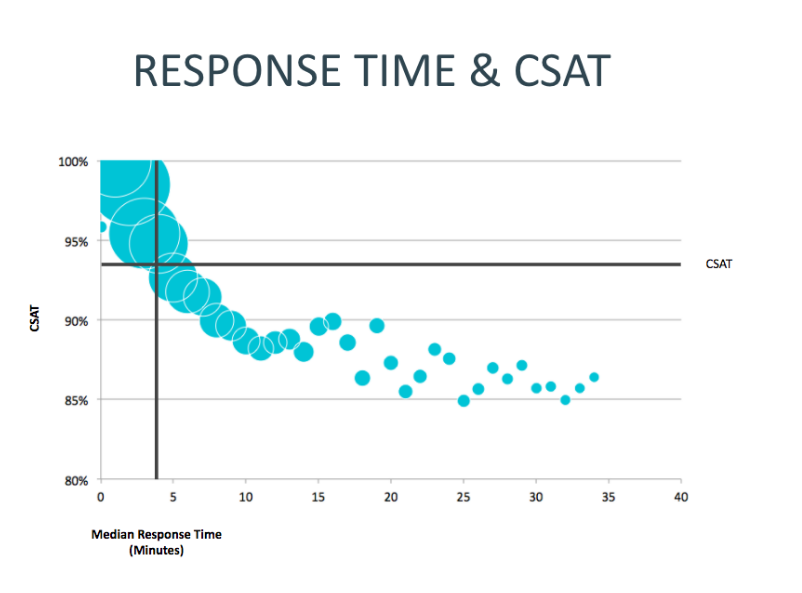
\includegraphics{figures/CSAT.png}\footnote{\tiny{}CSAT Figure - https://www.linkedin.com/pulse/faster-response-times-linked-high-csat-peter-thalman}}
				\end{center}
			\end{figure}
		\end{frame}
		%/////////////////////////////////////////////////
		\section{Qpid-Dispatch}
		\begin{frame}{Qpid-Dispatch}
				\begin{itemize}
						\setlength\itemsep{0.5em}
						\item Application layer router. 
						\item Take care of message routing in the network.
						\item Communication with Messaging Broker and Messaging Clients.		
						\item Each router has configuration file with specified links to other components.
						\item Network with routers can be configured with redundant links in case of any node crash.
				\end{itemize}						
		\end{frame}
		%/////////////////////////////////////////////////
		\section{Messaging Performance Tool}
		\begin{frame}{Messaging Performance Tool}
       		\begin{tabular}{cl}  
           		\begin{tabular}{l}
             		\parbox{0.37\linewidth}{%  change the parbox width as appropiate
						\begin{itemize}
							\setlength\itemsep{0.5em}
							\item Cluster performance testing system
							\item Load handlers are Sender and Receiver
							\item Inspector is monitoring component
							\item Communication between back-end and Maestro Clients through Maestro Broker
							\item Measured data are send to data server from Inspector
						\end{itemize}
   					}
         		\end{tabular} 
         		& \begin{tabular}{l}
           			\scalebox{0.32}{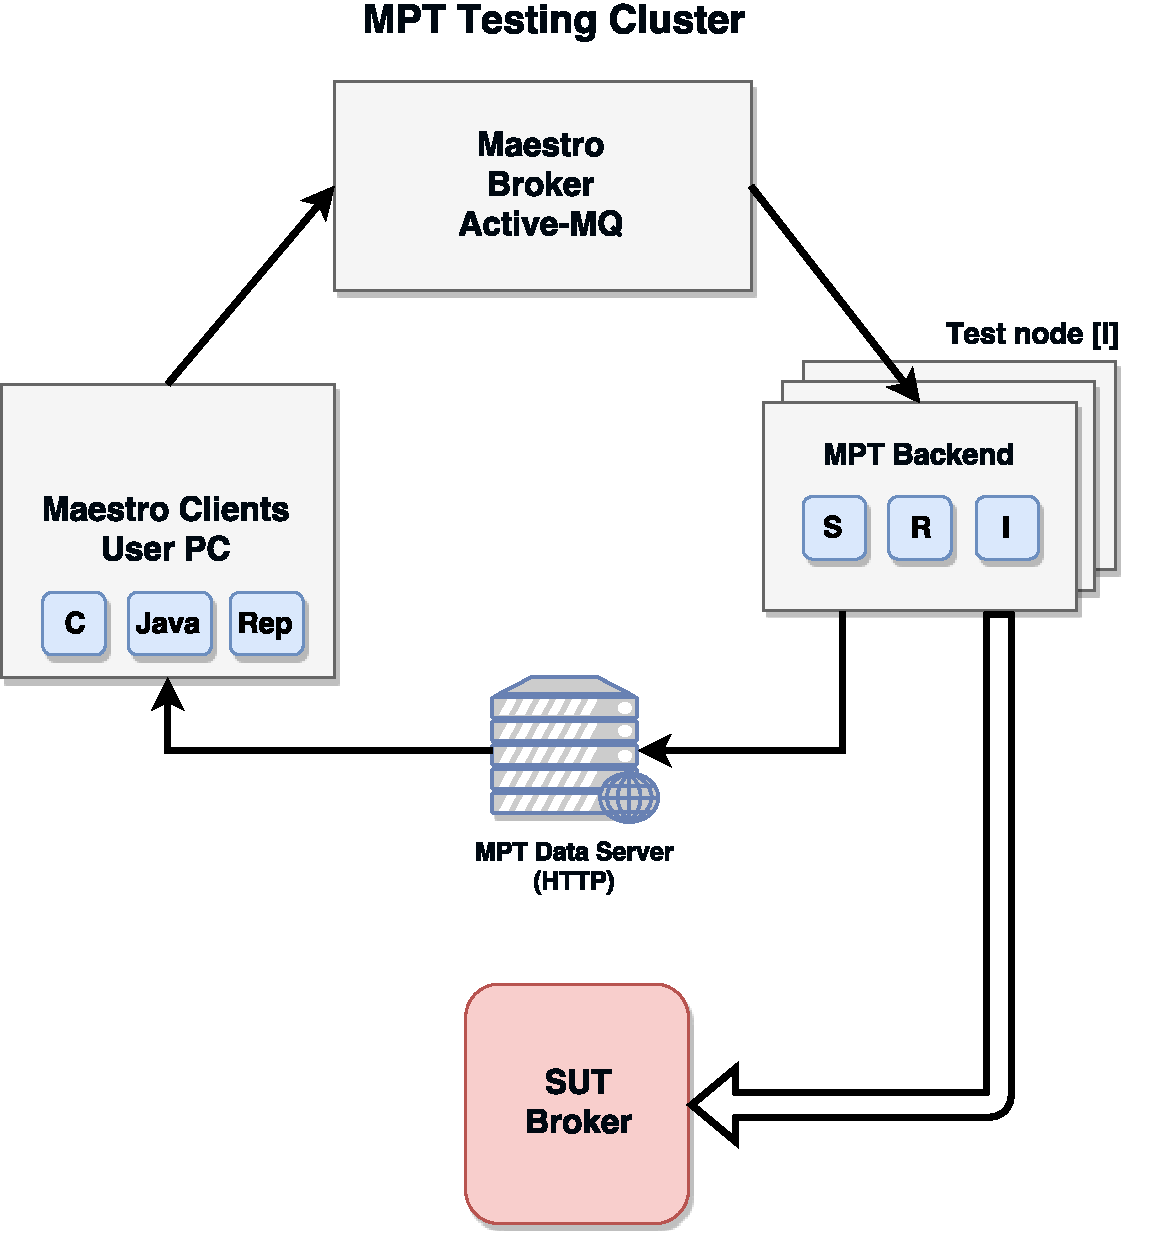
\includegraphics{figures/msg_perf_tool.pdf}}
           		\end{tabular} \\
			\end{tabular}					
		\end{frame}
		%/////////////////////////////////////////////////
		\section{Messaging Performance Tool: Proposed Extension}
		\begin{frame}{Messaging Performance Tool: Proposed Extension}
       		\begin{tabular}{cl}  
           		\begin{tabular}{l}
             		\parbox{0.37\linewidth}{%  change the parbox width as appropiate
						\begin{itemize}
							\setlength\itemsep{0.5em}
							\item Maestro Clients update (New Commands)
							\item New component: Agent
							\item Ability to change topology (Shut down router, etc.)
							\item Finished work:
							\vspace{0.5em}
							\begin{itemize}
								\setlength\itemsep{0.5em}
								\item Updated Maestro Clients with new commands
								\item Updated Maestro Broker with new topics
								\item Implemented Agent component
							\end{itemize}
						\end{itemize}
   					}
         		\end{tabular} 
         		& \begin{tabular}{l}
           			\scalebox{0.32}{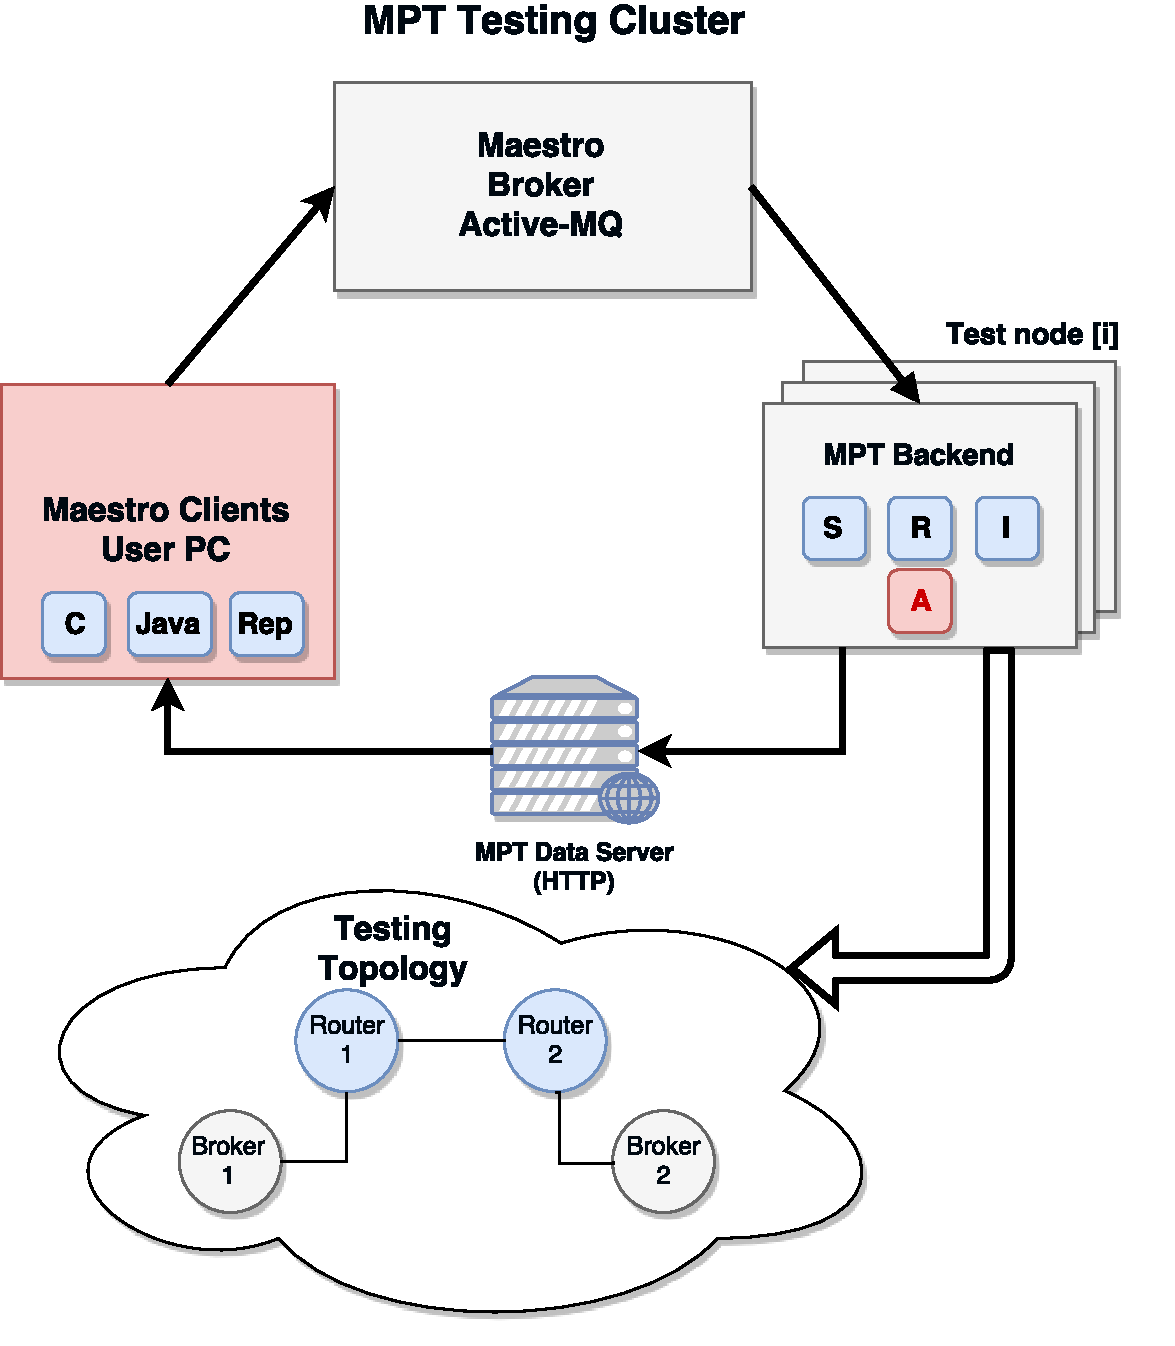
\includegraphics{figures/msg_perf_tool_for_router.pdf}}
           		\end{tabular} \\
			\end{tabular}	
		\end{frame}		
		%/////////////////////////////////////////////////
		\section{Topology Generator}
		\begin{frame}{Topology Generator}
       		\begin{tabular}{cl}  
           		\begin{tabular}{l}
             		\parbox{0.4\linewidth}{%  change the parbox width as appropiate
						\begin{itemize}
							\setlength\itemsep{0.5em}						
							\item Metadata are transformed into Configuration files
							\item Metadata consists of Inventory or Graph File (topology description)
							\item Configuration files are based on Qpid-Dispatch version (specific Template for Ansible)
							\item Automatic deployment of configuration files by Ansible to specific nodes
						\end{itemize}
   					}
         		\end{tabular} 
         		& \begin{tabular}{l}
           			\scalebox{0.3}{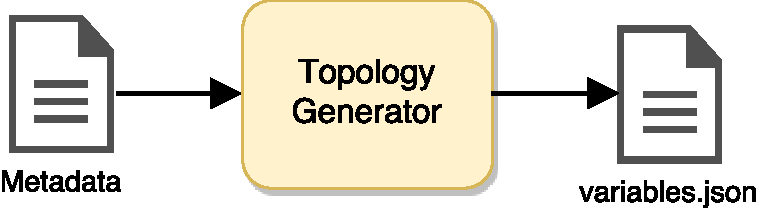
\includegraphics{figures/generator.pdf}} \\ \\ \\
           			\scalebox{0.3}{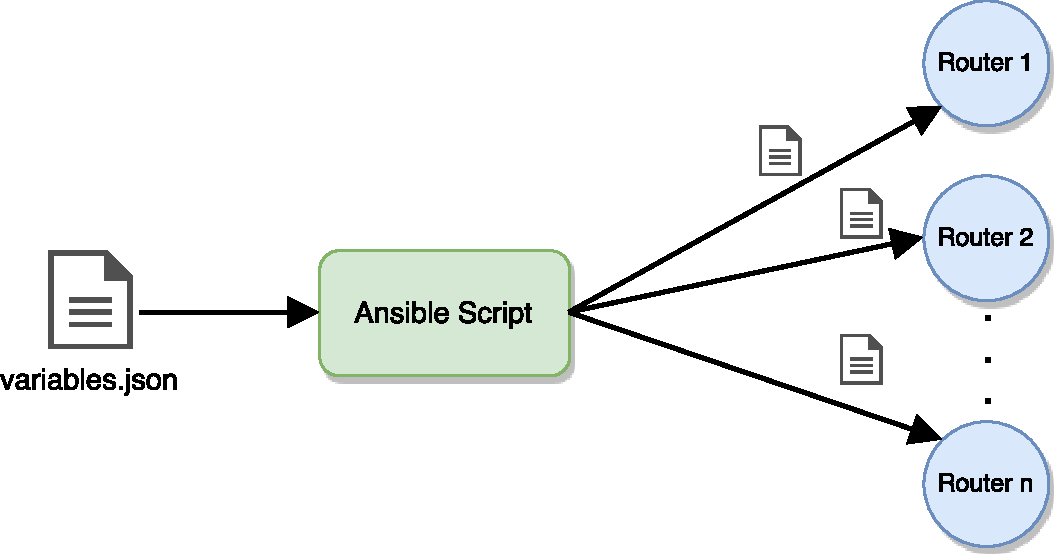
\includegraphics{figures/deployment.pdf}}
           		\end{tabular} \\
			\end{tabular}						
		\end{frame}
		%/////////////////////////////////////////////////
		\section{Summary}
		\begin{frame}{Summary}
				\begin{itemize}
						\setlength\itemsep{0.5em}
						\item Extension of Messaging Performance Tool
						\vspace{0.5em}
						\begin{itemize}
							\setlength\itemsep{0.5em}
							\item Added new commands to Maestro Clients
							\item Implemented Qpid-Dispatch Agent
						\end{itemize}
						\item Plan for next semester
						\vspace{0.5em}
						\begin{itemize}
							\setlength\itemsep{0.5em}
							\item Improvements of Topology Generator (more user friendly input, more default graphs)
							\item Qpid-Dispatch performance measurements (measure the highest throughput and other metrics)
							\item Experiments with Qpid-Dispatch recovery and topology convergence
						\end{itemize}
				\end{itemize}
		\end{frame}
		%/////////////////////////////////////////////////
\end{document}